\DiaryEntry{CRC Check Codes}{2015-06-28}{Maths}

A good description of CRC codes/checks can be found here
\url{http://www.ross.net/crc/download/crc_v3.txt}

I'm using a generator polynomial \(x^3 + x + 1\) which is equivalent to
\texttt{1011}.

\subsection{Encoding Example}\label{encoding-example}

As an example, consider encoding of the dataword =
\texttt{110100\ 1110\ 1100}. With the choice of the generator polynomial
as above, the CRC check code will have 3 digits, therefore we augment 3
zeros to the dataword. Then we divide the augmented dataword by the
generator polynomial.

\begin{figure}[hbt!]
\centering
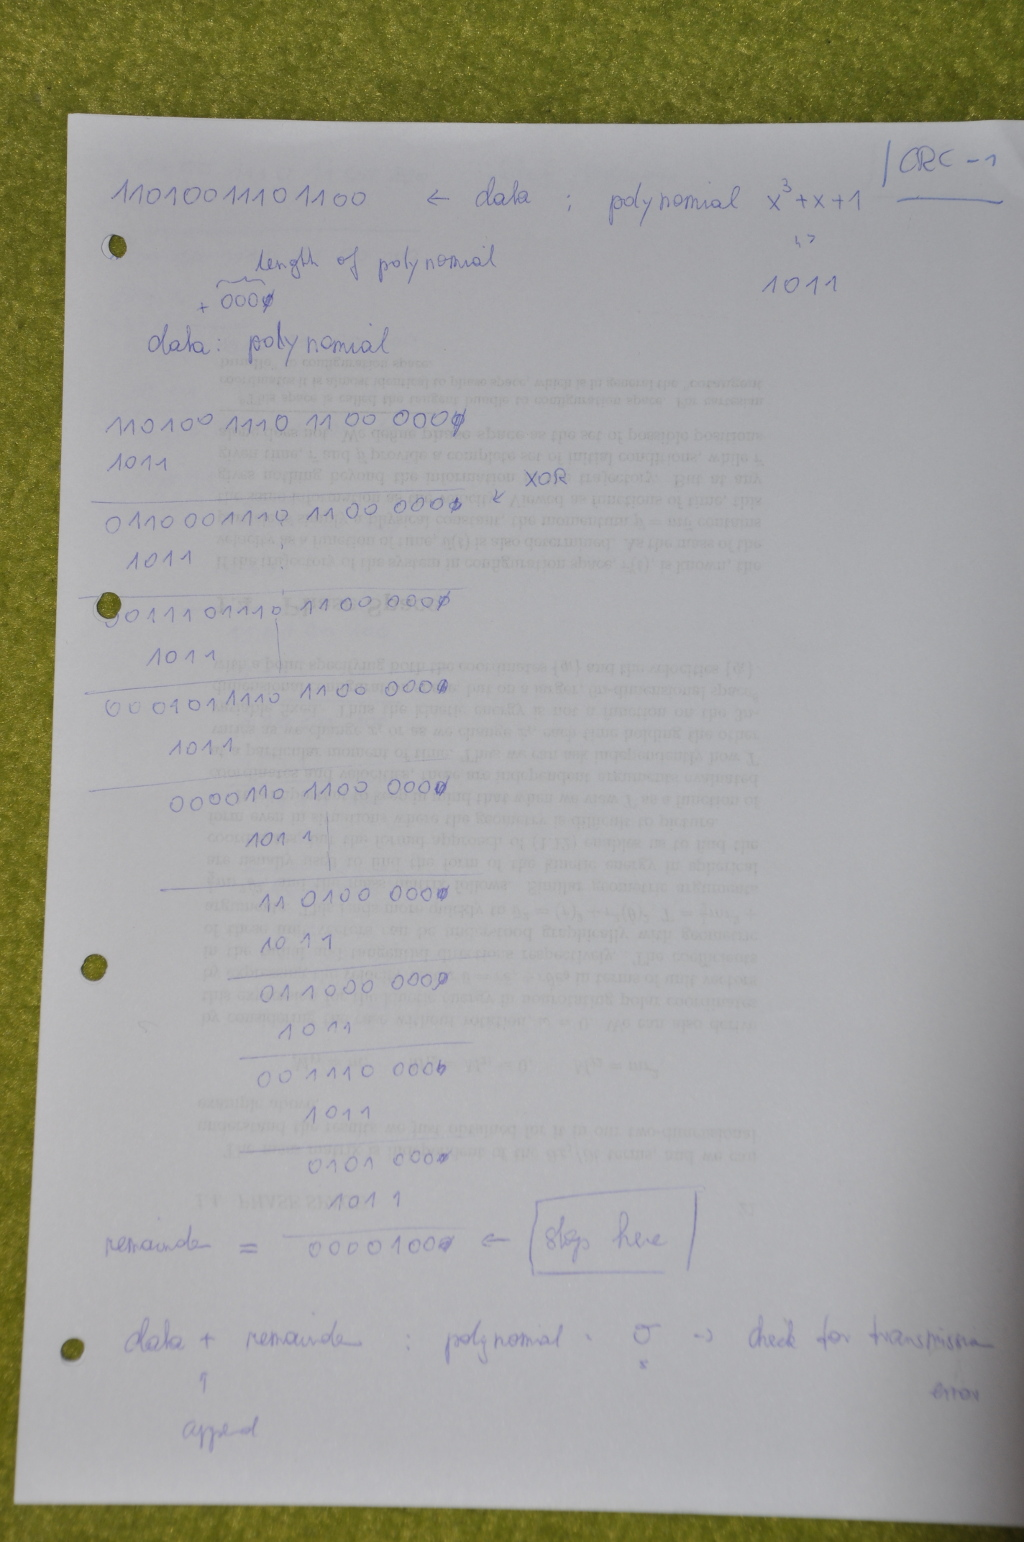
\includegraphics[scale=1.2]{images/DSC_0855_small.JPG}
\end{figure}

Division yields a remainder of \texttt{100} which is the CRC code. We
augment the original dataword with the CRC code to obtain
\texttt{11\ 0100\ 1110\ 1100\ 100}.

\subsection{Decoding Example}\label{decoding-example}

We divide the augmented dataword by the generator polynomial. In case of
no transmission errors, this should yield zero.

\begin{figure}[hbt!]
\centering
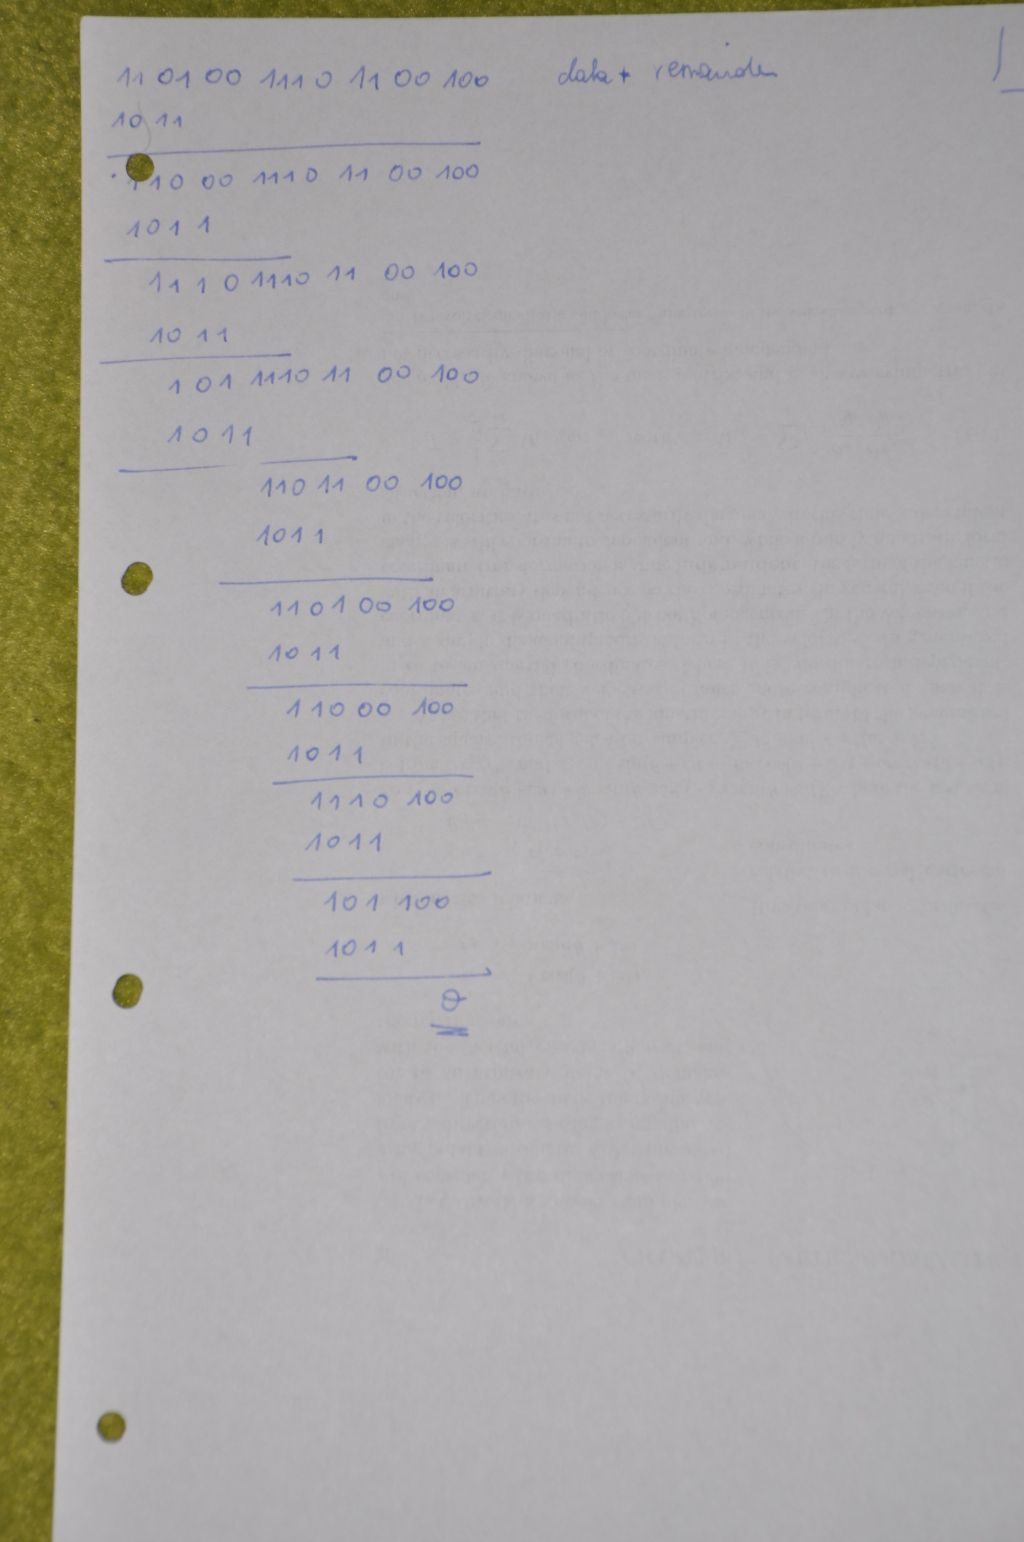
\includegraphics[scale=1.2]{images/DSC_0856_small.JPG}
\end{figure}

\subsection{Julia Example}\label{julia-example}

The (unofficial) Julia Module \texttt{IntModN} provides polynomial
arithmetic over GFs. Below is the example from above solved using this
module.

\begin{verbatim}
include("IntModN.jl")

x=IntModN.X(IntModN.GF2)

w = x^13 + x^12 + x^10 + x^7 + x^6 + x^5 + x^3 + x^2

dw_aug = dw * x^3

# crc code polynomial
p2 = x^3 + x + 1

println(dw_aug)
println(p2)

# divide with remainder; b holds the crc checkword
a, b = IntModN.divrem(dw_aug, p2)

println(a, " ... " , b)

# we finally transmit the dataword augmented with the crc checkword
dw_final = dw_aug + b

# dividing the received dataword by the crc polynomial
c, d = IntModN.divrem(dw_final, p2)

# yields a remainder of zero
println(d)
\end{verbatim}
